\documentclass[12pt]{report}
\usepackage[utf8]{inputenc}
\usepackage{geometry}
\geometry{letterpaper, margin=0.25in}
\usepackage{graphicx} 
\usepackage{multicol}
\usepackage{parskip}
\usepackage{booktabs}
\usepackage{array} 
\usepackage{paralist} 
\usepackage{verbatim}
\usepackage{sectsty}
\usepackage[shortlabels]{enumitem}

\usepackage{amsmath}
\usepackage{amssymb}
\usepackage{mathtools}
\usepackage{empheq}
\usepackage{xcolor}
\usepackage{bbm}
\usepackage{tikz}
\usepackage{pgfplots}
\usepackage{tikz-cd}
\usepackage{circuitikz}
\usepackage{multirow}

\usepackage[numbered,framed]{matlab-prettifier}
\lstset{
  style              = Matlab-editor,
  basicstyle         = \fontencoding{T1}\fontfamily{zi4}\selectfont\small, % Inconsolata, close to MATLAB's editor font
  numberstyle        = \fontencoding{T1}\fontfamily{zi4}\selectfont\scriptsize\color{gray},
  escapechar         = ",
  mlshowsectionrules = true,
}

\pgfplotsset{compat=1.18}
\usepgfplotslibrary{groupplots}
\usetikzlibrary{intersections, decorations.markings}
\tikzset{
    marking along/.style n args={2}{
        decoration={
                markings, 
                mark=at position #1 with {\arrow{#2}}
        },
        postaction={decorate}
        },
    marking along/.default={0.5}{>}
    wavy/.style={
        decorate,decoration={coil,aspect=0}
     },
    two marks/.style n args={1}{
        decoration={
            markings,
            mark=at position 0.25 with {\arrow{#1}},
            mark=at position 0.75 with {\arrow{#1}}
         },
         postaction={decorate}
    }
    two marks/.default={>}
}

% ---- Block diagram styles ----
% Usage: \begin{tikzpicture}[blockdiagram] ... place nodes relative to each other
% with right=of / below=of, then connect them by name. See the PID example.
\usetikzlibrary{arrows.meta, positioning, calc, patterns, decorations.pathmorphing}
\tikzset{
    blockdiagram/.style={>=Stealth, thick, font=\small, node distance=1cm and 1.5cm},
    block/.style={draw, minimum width=2.4cm, minimum height=1.2cm, align=center},
    sum/.style={draw, circle, minimum size=0.7cm, inner sep=0pt},
    branch/.style={fill, circle, inner sep=1.5pt},
    input/.style={coordinate},
    output/.style={coordinate},
    % sign labels for a summing junction: put on the arrow entering the sum
    plus/.style={pos=0.9, below left},
    minus/.style={pos=0.9, below right},
}

\colorlet{mygreen}{green!50!teal}
\colorlet{darkblue}{blue!60!black}

\newcommand{\ans}[1]{\boxed{\text{#1}}}
\newcommand{\vecs}[1]{\langle #1\rangle}
\renewcommand{\hat}[1]{\widehat{#1}}

\renewcommand{\P}{\mathbb{P}}
\newcommand{\R}{\mathbb{R}}
\newcommand{\E}{\mathbb{E}}
\newcommand{\Z}{\mathbb{Z}}
\newcommand{\N}{\mathbb{N}}
\newcommand{\Q}{\mathbb{Q}}
\newcommand{\C}{\mathbb{C}}

\newcommand{\ind}{\mathbbm{1}}
\newcommand{\qed}{\quad \blacksquare}

\newcommand{\brak}[1]{\left\langle #1 \right\rangle}
\newcommand{\bra}[1]{\left\langle #1 \right\vert}
\newcommand{\ket}[1]{\left\vert #1 \right\rangle}

\newcommand{\abs}[1]{\left\vert #1 \right\vert}
\newcommand{\mfX}{\mathfrak{X}}
\newcommand{\ep}{\varepsilon}

\newcommand{\Ec}{\mathcal{E}}
\newcommand{\Nc}{\mathcal{N}}
\newcommand{\A}{\mathcal{A}}
\newcommand{\F}{\mathcal{F}}
\newcommand{\Cc}{\mathcal{C}}
\newcommand{\B}{\mathcal{B}}
\newcommand{\M}{\mathcal{M}}
\newcommand{\X}{\chi}
\renewcommand{\L}{\mathcal{L}}

\newcommand{\sub}{\subseteq}
\newcommand{\st}{\text{ s.t. }}
\newcommand{\card}{\text{card }}
\renewcommand{\div}{\vspace*{10pt}\hrule\vspace*{10pt}}
\newcommand{\surj}{\twoheadrightarrow}
\newcommand{\inj}{\hookrightarrow}
\newcommand{\biject}{\hookrightarrow \hspace{-8pt} \rightarrow}
\renewcommand{\bar}[1]{\overline{#1}}
\newcommand{\overcirc}[1]{\overset{\circ}{#1}}
\newcommand{\diam}{\text{diam }}
\newcommand{\iid}{\overset{	ext{iid}}{\sim}}

\renewcommand{\Re}{\text{Re}\,}
\renewcommand{\Im}{\text{Im}\,}
\newcommand{\Var}{\text{Var}\,}
\newcommand{\Cov}{\text{Cov}\,}

\renewcommand{\tt}[1]{\texttt{#1}}

\DeclareMathOperator*{\argmax}{\arg\max}
\DeclareMathOperator*{\argmin}{\arg\min}

\newcommand{\sign}{\text{sign}\,}

\newcommand*{\tbf}[1]{\ifmmode\mathbf{#1}\else\textbf{#1}\fi}

\usepackage{tcolorbox}
\tcbuselibrary{breakable, skins}
\tcbset{enhanced}
\newenvironment*{tbox}[2][gray]{
    \begin{tcolorbox}[
        parbox=false,
        colback=#1!5!white,
        colframe=#1!75!black,
        breakable,
        title={#2}
    ]}
    {\end{tcolorbox}}

\newenvironment*{exercise}[1][red]{
    \begin{tcolorbox}[
        parbox=false,
        colback=#1!5!white,
        colframe=#1!75!black,
        breakable
    ]}
    {\end{tcolorbox}}

\newenvironment*{proof}[1][blue]{
\begin{tcolorbox}[
    parbox=false,
    colback=#1!5!white,
    colframe=#1!75!black,
    breakable
]}
{\end{tcolorbox}}
\newenvironment*{proposition}[1][gray]{
    \begin{tcolorbox}[
        parbox=false,
        colback=#1!5!white,
        colframe=#1!75!black,
        breakable
    ]}
    {\end{tcolorbox}}


\title{ENGN 1931Y: Control Systems Engineering}
\author{Milan Capoor}
\date{Fall 2026}
\begin{document}
\maketitle 

\section{Sept 10}

\tbf{Control system:} a mechanism that alters the future state of a system

\tbf{Control theory:} a strategy to achieve the desired system performance 
\begin{itemize}
    \item Alternatively, the study of how to regulate and manage the behavior of dynamic system using feedback control loop
\end{itemize}

\section{Feb 15}
\tbf{Types of Control Systems}
\begin{itemize}
    \item Logic control (e.g. programmable logic controller) 
    \item On-off control (e.g. light switch)
    \item Feedback control 
\end{itemize}

In this class we will focus on feedback control systems and represent almost everything with block diagrams abstracting the system into inputs and outputs.

\emph{Example:} A car block diagram

\begin{center}
\begin{tikzpicture}
    \draw (0, 0) rectangle ++(3, 3) node[midway]{Plant};
    \draw[<-] (0, 1.5) -- ++(-2, 0) node[midway, above]{Throttle};
    \draw[->] (3, 1.5) -- ++(2, 0) node[midway, above]{Velocity};
\end{tikzpicture}
\end{center}

\tbf{Open loop control:} system without feedback. 
\begin{itemize}
    \item In the car example, we can imagine a cruise control system that sets the throttle to a fixed value. Without incorporating knowledge of dynamics or feedback, we cannot compensate for uncertain masses, varying environmental controls, or imprecise models
\end{itemize}

\tbf{Closed loop control:} system with feedback used to control despite our incomplete knowledge (though this trades off stability, response speed, etc.)
\begin{itemize}
    \item In the car example, we update the throttle command based on a measurement of the current speed
\end{itemize}

\begin{center}
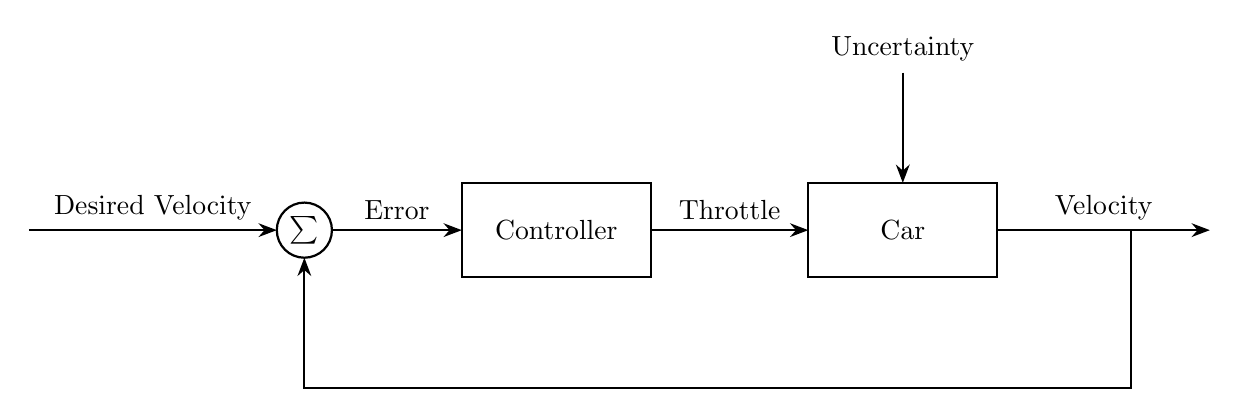
\begin{tikzpicture}[>=Stealth, thick]
    \draw (0,0) circle (0.35) node[midway] {$\sum$};

    \draw[->] (-3.5,0) -- (-0.35,0) node[midway, above] {Desired Velocity};

    \draw[->] (0.35,0) -- (2,0) node[midway, above] {Error};

    \draw (2,-0.6) rectangle ++(2.4,1.2) node[midway] {Controller};

    \draw[->] (4.4,0) -- (6.4,0) node[midway, above] {Throttle};

    \draw (6.4,-0.6) rectangle ++(2.4,1.2) node[midway] {Car};

    \draw[->] (7.6,2) -- (7.6,0.6);
    \node at (7.6,2.3) {Uncertainty};

    \draw[->] (8.8,0) -- (11.5,0) node[midway, above] {Velocity};

    \draw[->] (10.5,0) -- (10.5,-2) -- (0,-2) -- (0,-0.35);
\end{tikzpicture}
\end{center}


Any block diagram must involve:
\begin{itemize}
    \item Desired reference
    \item Controller
    \item Plant
    \item Sensor 
    \item Feedback
    \item Uncertainty
\end{itemize}

\tbf{Example:} Consider the system in a car where 1 degree throttle change maps to 10 mph change in speed and a 1\% change in road grade maps to -5 mph change in speed. How do we relate road grade to throttle change? (Trivially, 1\% change equals 0.5 degree throttle)

How might we draw this controller? 

\begin{center}
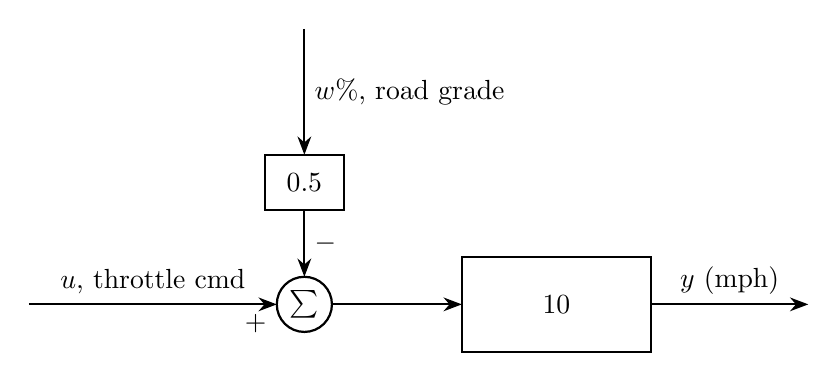
\begin{tikzpicture}[>=Stealth, thick]
    \draw (0,0) circle (0.35) node[midway] {$\sum$};

    \draw[->] (-3.5,0) -- (-0.35,0) node[midway, above] {$u$, throttle cmd} node[below left] {$+$};

    \draw[->] (0, 1.2) -- (0, 0.35) node[midway, right] {$-$};
    \draw (-0.5, 1.2) rectangle ++(1, 0.7) node[midway] {0.5};
    \draw[->] (0, 3.5) -- (0, 1.9) node[midway, right] {$w\%$, road grade};

    \draw[->] (0.35,0) -- (2,0);
    \draw (2,-0.6) rectangle ++(2.4,1.2) node[midway] {10};
    \draw[->] (4.4,0) -- (6.4,0) node[midway, above] {$y$ (mph)};


\end{tikzpicture}
\end{center}

The naive open loop controller ignores the disturbance and simply maps the desired speed to $1/10$ of that value in throttle so $r = y$ if $w = 0$. 

\begin{center}
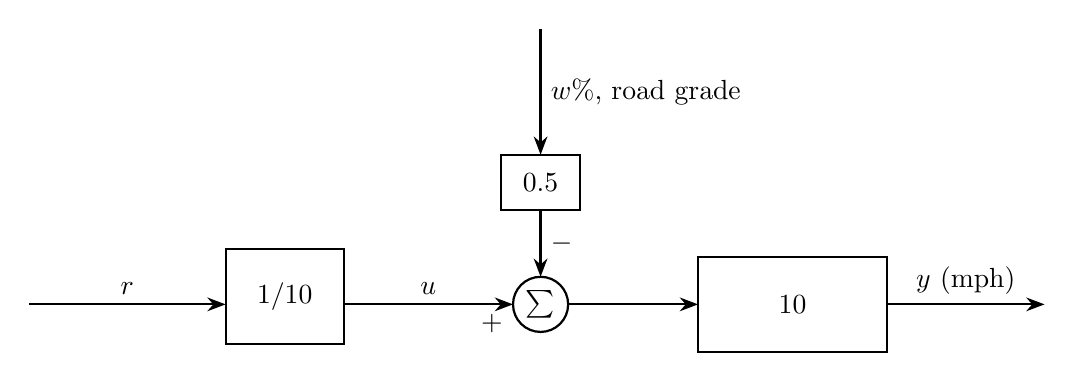
\begin{tikzpicture}[>=Stealth, thick]
    \draw (0,0) circle (0.35) node[midway] {$\sum$};

    \draw[->] (-2.5,0) -- (-0.35,0) node[midway, above] {$u$} node[below left] {$+$};

    \draw[->] (0, 1.2) -- (0, 0.35) node[midway, right] {$-$};
    \draw (-0.5, 1.2) rectangle ++(1, 0.7) node[midway] {0.5};
    \draw[->] (0, 3.5) -- (0, 1.9) node[midway, right] {$w\%$, road grade};

    \draw[->] (0.35,0) -- (2,0);
    \draw (2,-0.6) rectangle ++(2.4,1.2) node[midway] {10};
    \draw[->] (4.4,0) -- (6.4,0) node[midway, above] {$y$ (mph)};

    \draw (-4, -0.5) rectangle ++(1.5, 1.2) node[midway] {$1/10$};
    \draw[<-] (-4, 0) -- ++(-2.5, 0) node[midway, above] {$r$ };

\end{tikzpicture}
\end{center}

Hence the actual control exerted is
\begin{align*}
    y &= r - 0.5 (10) w\\ 
    &= r - 5w\\ 
    e &= r - y\\ 
    &= r - (r - 5w)\\
    &= 5w
\end{align*}
so our \% speed error is $500w/r$. At $r = 65$ mph and $w = 1\%$, we have a 7.7\% error in speed.

\tbf{Remark:} in this example we had to choose $1/10$ as the gain of the controller to achieve $r = y$ when $w = 0$. This required knowledge of the plant dynamics. In general, we may not know the plant dynamics and hence cannot choose a controller gain to achieve this. This motivates the use of feedback control.

Let's try this again with feedback control. 

\begin{center}
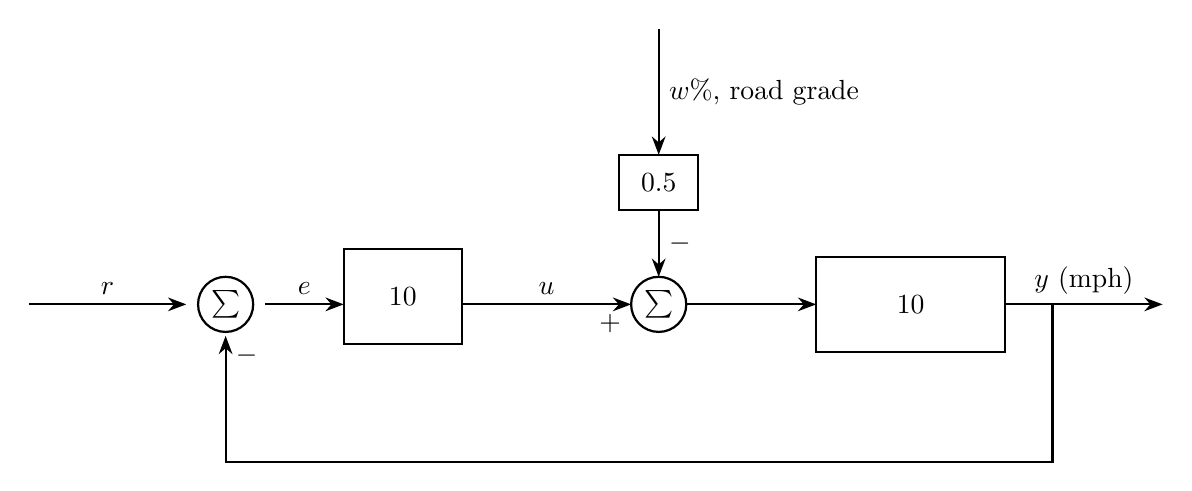
\begin{tikzpicture}[>=Stealth, thick]
    \draw (0,0) circle (0.35);
    \node at (0,0) {$\sum$};

    \draw[->] (-2.5,0) -- (-0.35,0) node[midway, above] {$u$} node[below left] {$+$};

    \draw[->] (0, 1.2) -- (0, 0.35) node[midway, right] {$-$};
    \draw (-0.5, 1.2) rectangle ++(1, 0.7) node[midway] {0.5};
    \draw[->] (0, 3.5) -- (0, 1.9) node[midway, right] {$w\%$, road grade};

    \draw[->] (0.35,0) -- (2,0);
    \draw (2,-0.6) rectangle ++(2.4,1.2) node[midway] {10};
    \draw[->] (4.4,0) -- (6.4,0) node[midway, above] {$y$ (mph)};

    \draw (-4, -0.5) rectangle ++(1.5, 1.2) node[midway] {$10$};

    \draw (-5.5,0) circle (0.35);
    \node at (-5.5,0) {$\sum$};
    \draw[<-] (-6, 0) -- ++(-2, 0) node[midway, above] {$r$ };
    \draw[->] (-5, 0) -- ++(1, 0) node[midway, above] {$e$};

    \draw[->] (5, 0) -- ++(0, -2) -- ++(-10.5, 0) -- ++(0, 1.6) node[below right] {$-$};


\end{tikzpicture}
\end{center}

If we arbitrarily set the gain at $10$, our system is governed by 
\[\begin{cases}
    y = 10 (u - 0.5 w)\\ 
    u = 10(r - y)
\end{cases} \implies y = 100r - 100y - 5w \implies y = \frac{100}{101}r  - \frac{5}{101}w \approx 0.99r - 0.05w\]

If $w=1$ and $r = 65$,
\[e = y -r = \frac{r}{101} + \frac{5}{101}w\]
and the error percentage is 
\[e\% = \frac{100e}{r} = \frac{0.01r - 0.05}{r} \approx 0.076\% \]

What if we set the gain to $1000$? Wouldn't that send the error to $0.0007\%$? Not necessarily. This can lead to instability and oscillations. 

\tbf{Example:} Consider a house with a heater and a thermostat. 

\begin{center}
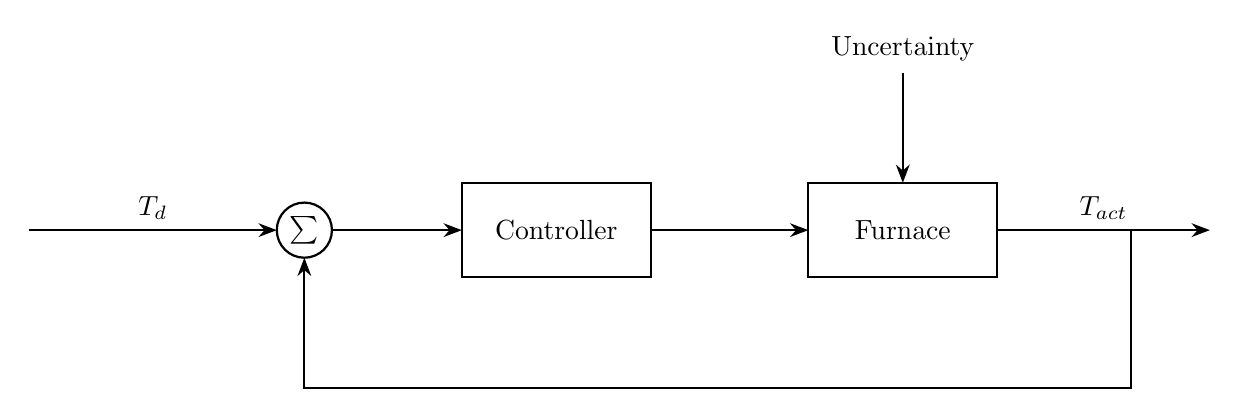
\begin{tikzpicture}[>=Stealth, thick]
    \draw (0,0) circle (0.35) node[midway] {$\sum$};

    \draw[->] (-3.5,0) -- (-0.35,0) node[midway, above] {$T_d$};

    \draw[->] (0.35,0) -- (2,0);

    \draw (2,-0.6) rectangle ++(2.4,1.2) node[midway] {Controller};

    \draw[->] (4.4,0) -- (6.4,0);

    \draw (6.4,-0.6) rectangle ++(2.4,1.2) node[midway] {Furnace};

    \draw[->] (7.6,2) -- (7.6,0.6);
    \node at (7.6,2.3) {Uncertainty};

    \draw[->] (8.8,0) -- (11.5,0) node[midway, above] {$T_{act}$};

    \draw[->] (10.5,0) -- (10.5,-2) -- (0,-2) -- (0,-0.35);
\end{tikzpicture}
\end{center}

\[e = T_d - T_{act}\]

Notice here the furnace can only turn on and off so we have a delay in the system response. This results in the actual temperature sawtoothing around the setpoint:

\begin{center}
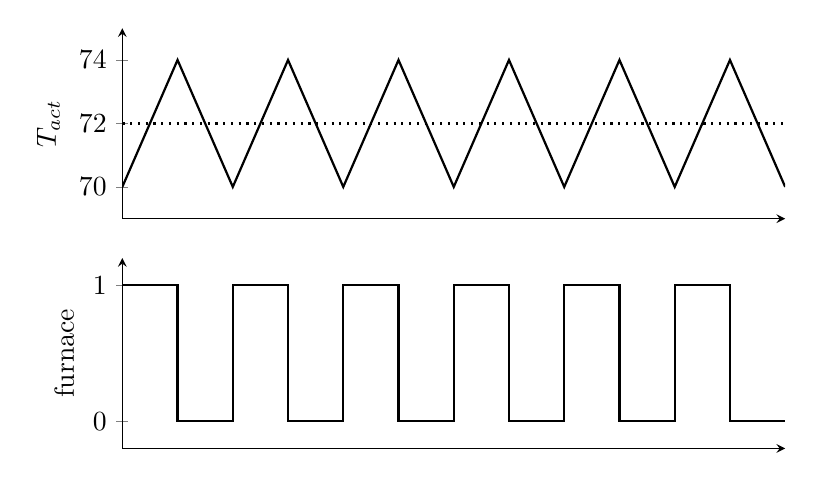
\begin{tikzpicture}
    \begin{groupplot}[
        group style={group size=1 by 2, vertical sep=0.5cm},
        width=10cm, height=4cm,
        xmin=0, xmax=12,
        xtick=\empty,
        axis lines=left,
    ]
    \nextgroupplot[ymin=69, ymax=75, ylabel={$T_{act}$}]
        \addplot[dotted, thick, domain=0:12, samples=2] {72};
        \addplot[thick] coordinates {
            (0,70) (1,74) (2,70) (3,74) (4,70) (5,74)
            (6,70) (7,74) (8,70) (9,74) (10,70) (11,74) (12,70)
        };
    \nextgroupplot[ymin=-0.2, ymax=1.2, ytick={0,1}, ylabel={furnace}]
        \addplot[thick] coordinates {
            (0,1) (1,1) (1,0) (2,0)
            (2,1) (3,1) (3,0) (4,0)
            (4,1) (5,1) (5,0) (6,0)
            (6,1) (7,1) (7,0) (8,0)
            (8,1) (9,1) (9,0) (10,0)
            (10,1) (11,1) (11,0) (12,0)
        };
    \end{groupplot}
\end{tikzpicture}
\end{center}

\section{Sept 17}

\tbf{Recall:} last time we introduced a general block diagram for a \emph{Single-input single-output} (SISO) feedback control system.

\begin{center}
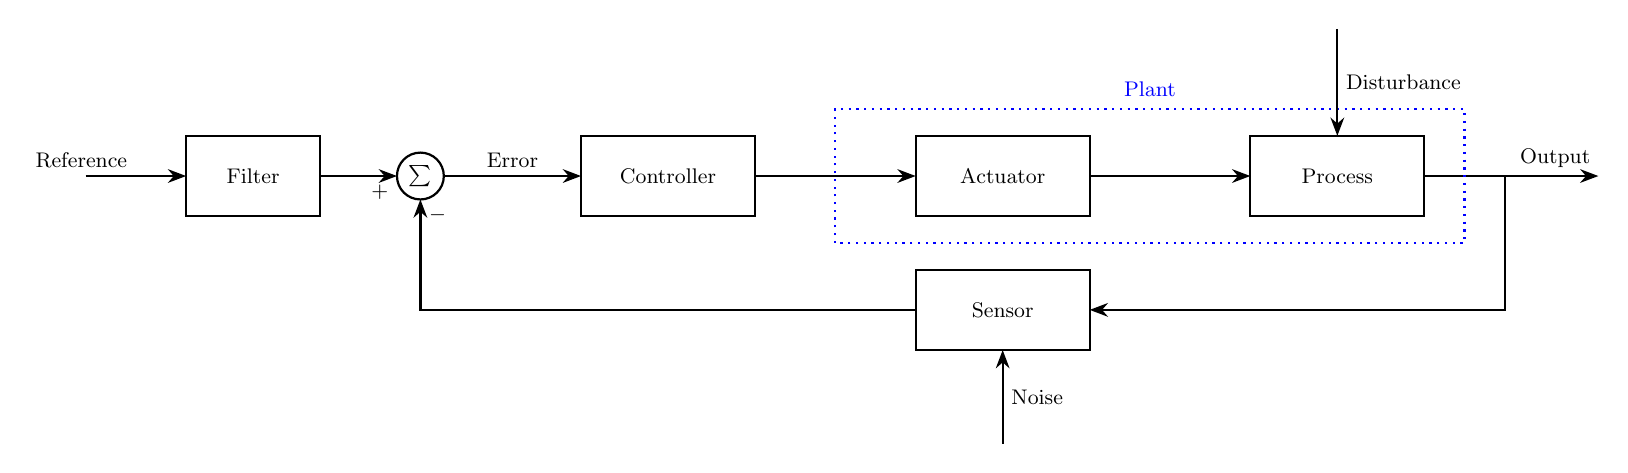
\begin{tikzpicture}[>=Stealth, thick, scale=0.85, every node/.style={transform shape}, font=\small]
    \draw[->] (-5,0) -- (-3.5,0) node[midway, above left] {Reference};
    \draw (-3.5,-0.6) rectangle ++(2,1.2) node[midway] {Filter};

    \draw (0,0) circle (0.35) node[midway] {$\sum$};
    \draw[->] (-1.5,0) -- (-0.35,0) node[below left] {$+$};

    \draw[->] (0.35,0) -- (2.4,0) node[midway, above] {Error};

    \draw (2.4,-0.6) rectangle ++(2.6,1.2) node[midway] {Controller};
    \draw[->] (5,0) -- (7.4,0);

    \draw (7.4,-0.6) rectangle ++(2.6,1.2) node[midway] {Actuator};
    \draw[->] (10,0) -- (12.4,0);

    \draw (12.4,-0.6) rectangle ++(2.6,1.2) node[midway] {Process};
    \draw[->] (15,0) -- (17.6,0) node[midway, above right] {Output};

    \draw[blue, dotted, thick] (6.2,-1.0) rectangle (15.6,1.0);
    \node[blue] at (10.9,1.3) {Plant};

    \draw[->] (13.7,2.2) -- (13.7,0.6) node[midway, right] {Disturbance};

    \draw[->] (16.2,0) -- (16.2,-2) -- (10,-2);
    \draw (7.4,-2.6) rectangle ++(2.6,1.2) node[midway] {Sensor};
    \draw[->] (8.7,-4.0) -- (8.7,-2.6) node[midway, right] {Noise};
    \draw[->] (7.4,-2) -- (0,-2) -- (0,-0.35) node[below right] {$-$};
\end{tikzpicture}
\end{center}

\tbf{Characteristics of a well-designed control system:}
\begin{itemize}
    \item \emph{Stability}: the system should not diverge or oscillate uncontrollably
    \item \emph{Tracking}: the system should follow the desired reference accurately 
    \item \emph{Disturbance rejection}: the system should be able to maintain performance in the presence of disturbances
    \item \emph{Robustness}: the system should be able to handle model uncertainties and variations in system parameters
\end{itemize}

As we will see, each box in the block diagram can be represented by a mathematical model (in fact an ODE), and we can analyze the overall system behavior using these models.

\begin{proposition}
    \textbf{Laplace Transform:} for a bounded function $f(t)$, the Laplace transform is defined as
    \[\L[f(t)] = F(s) = \int_0^{\infty} f(t)\, e^{-st}\; dt\]
    where $s = \sigma + j\omega$ is a complex variable.  
\end{proposition}

(\emph{Remark:} we define the integral from $0$ to $\infty$ because we are only interested in causal systems, i.e. systems that do not depend on future inputs.)

\emph{Examples:} 

\begin{align*}
    \L[u(t)] &= 1/s &&(u(t) \text{ unit step function})\\
    \L[t u(t)] &= 1/s^2\\ 
    \L[t^2 u(t)] &= 1/s^3\\
    \L[\sin(\omega t) u(t)] &= \frac{\omega}{s^2 + \omega^2}\\
    \L[\cos(\omega t) u(t)] &= \frac{s}{s^2 + \omega^2}\\ 
    \L[\delta(t)] &= 1 &&(\delta(t) \text{ Dirac delta function})
\end{align*}

In Matlab, we can compute these transforms using the \tt{Symbolic Math Toolbox} and 
\begin{lstlisting}
    syms s t w
    Laplace(cos(w * t))
\end{lstlisting}

\tbf{Properties of the Laplace transform:}
\begin{enumerate}
    \item Linearity 
    \[\L[af(t) + bg(t)] = aF(s) + bG(s)\]
    \item Frequency shift 
    \[\L[e^{-at} f(t)] = F(s + a)\]
    \item Time shift 
    \[\L[f(t - T_d)] = F(s)e^{-T_d s}\]
    \item Scaling 
    \[\L[f(at)] = \frac{1}{a} F(\frac{s}{a})\]
    \item Integration/differentiation 
    \begin{align*}
        \L\left[\frac{d^nf(t)}{dt^n}\right] &= s^n F(s) + s^{n-1} f(0) + s^{n-2} f'(0) + \dots + f^{(n-1)}(0)\\
        \L\left[\int_0^t f(t)\; dt\right] &= \frac{1}{s} F(s)
    \end{align*}
    \item Behavior under convolution 
    \[\L[f(t) \star g(t)] = \L\left[\int_0^t f(t-\tau) g(\tau)\; dt\right] = F(s) G(s)\]

    \item Final/initial values
    \[\lim_{t \to \infty} f(t) = \lim_{s \to 0} sF(s)\]
\end{enumerate}

\emph{Proportional-Integral-Derivative Control:}
For $k_p, k_i, k_d \in \R$.
\begin{align*}
    u(t) &= k_p e(t) + k_i \int_0^t e(\tau)\; d\tau + k_d \frac{de(t)}{dt}\\ 
    U(s) &= k_p E(s) + k_i \frac{E(s)}{s} + k_d s E(s)\\
\end{align*}

Notice by grouping terms, 
\[\frac{U(s)}{E(s)} = \frac{k_d s^2 + k_p s + k_i}{s}\]
so by using the Laplace transform, we can represent the PID controller as a polynomial transfer function 

\begin{center}
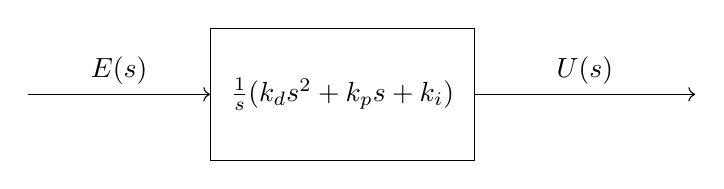
\begin{tikzpicture}[scale=1.4]

    \draw[->] (0.35,0) -- (2,0) node[midway, above] {$E(s)$};

    \draw (2,-0.6) rectangle ++(2.4,1.2) node[midway] {$\frac{1}{s}(k_d s^2 + k_p s + k_i)$};

    \draw[->] (4.4,0) -- (6.4,0) node[midway, above] {$U(s)$};
\end{tikzpicture}
\end{center}

\begin{exercise}
    \textbf{Exercise:}  Suppose there is a mass-on-spring system governed by 
    \[F = M \ddot x + c \dot x + kx\]
    What is the transfer function?

    \div 

    \begin{align*}
        \L[F] &= M (s^2 X(s) - s x(0) - x'(0)) + c (s X(s) - x(0)) + k X(s)\\ 
        &= (Ms^2  + cs + k)X(s)\\ 
        \frac{X(s)}{F(s)} &= \frac{1}{Ms^2 + cs + k}
    \end{align*}
    
\end{exercise}

This will allow us to control the system by a simple block diagram

\begin{center}
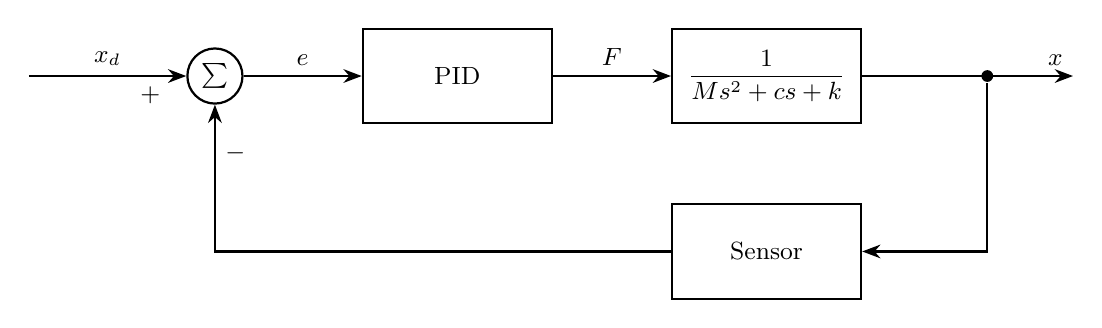
\begin{tikzpicture}[blockdiagram]
    % nodes: position each relative to the previous one
    \node[input]                        (in)     {};
    \node[sum, right=2cm of in]         (sum)    {$\sum$};
    \node[block, right=of sum]          (ctrl)   {PID};
    \node[block, right=of ctrl]         (plant)  {$\dfrac{1}{Ms^2 + cs + k}$};
    \node[branch, right=1.5cm of plant] (split)  {};
    \node[output, right=1cm of split]   (out)    {};
    \node[block, below=of plant]        (sensor) {Sensor};

    % signals
    \draw[->] (in) -- node[above] {$x_d$} node[plus] {$+$} (sum);
    \draw[->] (sum) -- node[above] {$e$} (ctrl);
    \draw[->] (ctrl) -- node[above] {$F$} (plant);
    \draw[->] (plant) -- (out) node[above left] {$x$};

    % feedback
    \draw[->] (split) |- (sensor);
    \draw[->] (sensor) -| node[minus] {$-$} (sum);
\end{tikzpicture}
\end{center}

\section{Sept 22} 

\tbf{Example:} Use the Laplace transform to solve the following ODE:
\[\begin{cases}
    \ddot y + 5\dot y + 6y=0\\
    y(0) = 2\\ 
    \dot y = 3
\end{cases}\]

\begin{gather*}
    \L[\ddot y + 5 \dot y + 6y] = \L[0]\\ 
    s^2 Y(0) - sy(0) - \dot y(0) + 5(sY(s) - y(0)) + 6Y(s) = 0\\
    (s^2 + 5s + 6)Y(s) - 2s - 3 - 10 = 0\\ 
    Y(s) = \frac{2s + 13}{s^2 + 5s + 6}\\ 
    y(t) = \L^{-1}\left[\frac{2s + 13}{s^2 + 5s + 6}\right]
\end{gather*}

In this example, 
\[Y(s) = \frac{2s + 13}{s^2 + 5s + 6}\]
is our \tbf{transfer function}. We call the numerator our \tbf{zeroes} and the denominator our \tbf{poles}.

\subsection{Inverse Laplace Transform}
We use the \tbf{inverse laplace transform} to go from the transfer function back to the time domain.

In this problem, we need to use \emph{partial fractions}:
\begin{align*}
    \frac{2s + 13}{(s+2)(s+3)} &= \frac{A}{s+2} + \frac{B}{s+3}\\ 
    2s + 13 &= A(s+3) + B(s+2)\\ 
    2s + 13 &= (A+B)s + (3A + 2B)\\ 
    \begin{cases}
        A + B &= 2\\ 
        3A + 2B &= 13
    \end{cases} &\implies A = 9, B = -7\\ 
    y(t) &= \L^{-1}\left[\frac{9}{s+2} - \frac{7}{s+3}\right]\\
    &= \boxed{9 e^{-2t} - 7 e^{-3t}}
\end{align*}

\begin{center}
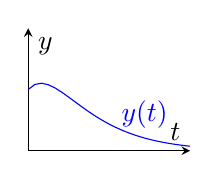
\begin{tikzpicture}
\begin{axis}[
    width=0.3\textwidth,
    axis lines=middle,
    no markers,
    xtick=\empty,
    ytick=\empty,
    clip=false,
    xlabel={$t$},
    ylabel={$y$},
    domain=0:2,
    ymin=0, ymax=4,
    xmin=0, xmax=2,
    view = {0}{90}
]
    \addplot{9*exp(-2*x) - 7*exp(-3*x)} node[pos=0.8, above] {$y(t)$};
\end{axis}
\end{tikzpicture}
\end{center}

\tbf{Example:}
\[F(s) = \frac{1}{s(s+0.1)^2} = \frac{K_1}{s} + \frac{K_2}{(s+0.1)^2} + \frac{K_3}{(s+0.1)}\]

Choosing $K_1$ and $K_2$ to cancel the denominators, we have
\begin{align*}
    K_1 &= \frac{1}{(0.1)^2} = 100\\
    K_2 &= \frac{1}{s}\bigg\vert_{s=-0.1} = -10\\
\end{align*}
and then for $K_3$ we just need to solve for the remaining constant. For ease of calculation, let $s = 1$:
\begin{align*}
     \frac{1}{s(s+0.1)^2} \bigg\vert_{s=1} &= \left[\frac{K_1}{s} + \frac{K_2}{(s+0.1)^2} + \frac{K_3}{(s+0.1)}\right]_{s=1}\\ 
    \frac{1}{1(1.1)^2} &= 100 + \frac{-10}{(1.1)^2} + \frac{K_3}{1.1}\\ 
    K_3 &= \frac{1}{1.1} - 100 + \frac{10}{(1.1)^2} \approx -90.74
\end{align*}

Note that when using partial fractions, we must have a term for each order of the repeated root.

This gives rise to a general transfer function of the form
\begin{align*}
    H(s) &= \frac{a_n s^n + a_{n-1}s^{n-1} + \dots + a_1}{s^m + b_{m-1}s^{m-1} + \dots + b_1}\\ 
    &= \frac{N(s)}{(s^2 + 2 \zeta \omega_n s + \omega_n^2)\prod_{j=3}^n \frac{1}{s - s_j}} 
\end{align*}

\tbf{Example:} With null initial conditions, the mass-spring-damper system is governed by
\[m\ddot x + c\dot x + kx = F(t)\]

\begin{center}
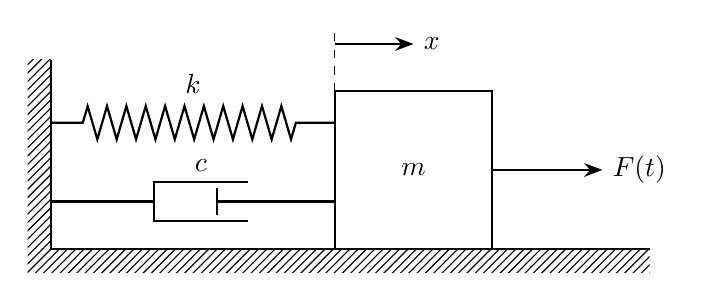
\begin{tikzpicture}[>=Stealth, thick]
    % wall and ground
    \fill[pattern=north east lines] (-0.3,0) rectangle (0,2.4);
    \fill[pattern=north east lines] (-0.3,-0.3) rectangle (7.6,0);
    \draw (0,2.4) -- (0,0) -- (7.6,0);

    % mass
    \draw (3.6,0) rectangle ++(2,2) node[midway] {$m$};

    % spring
    \draw[decoration={zigzag, segment length=7pt, amplitude=6pt, pre length=0.4cm, post length=0.4cm}, decorate]
        (0,1.6) -- (3.6,1.6) node[midway, above=7pt] {$k$};

    % damper
    \draw (0,0.6) -- (1.3,0.6);
    \draw (2.5,0.35) -- (1.3,0.35) -- (1.3,0.85) -- (2.5,0.85);
    \draw (2.1,0.43) -- (2.1,0.77);
    \draw (2.1,0.6) -- (3.6,0.6);
    \node[above] at (1.9,0.85) {$c$};

    % force
    \draw[->] (5.6,1) -- ++(1.4,0) node[right] {$F(t)$};

    % displacement
    \draw[dashed, thin] (3.6,2) -- (3.6,2.8);
    \draw[->] (3.6,2.6) -- ++(1,0) node[right] {$x$};
\end{tikzpicture}
\end{center}

The transfer function is 
\[\frac{X(s)}{F(s)} = \frac{1}{ms^2 + cs + k}\] 

We want to represent it as a \tbf{second order system} of the form 
\[s^2 + 2\zeta \omega_n s + \omega_n^2\]

Notice 
\[\frac{1}{ms^2 + cs + k} = \frac{1/m}{s^2 + \frac{c}{m}s + \frac{k}{m}}\]

Now $\omega_n = \sqrt{k/m}$ is the \tbf{natural frequency} while $2\zeta \omega_n = c/m$ is the \tbf{damping ratio}.

This second order form is essential because it allows us to decompose all higher order systems into a product of second order systems and first order systems.

Now consider the poles (the roots of the denominator $s^2 + 2\zeta \omega_n s + \omega_n^2$). What happens under different values of $\zeta$?

\[\begin{cases}
    \zeta = 0 &\implies s_{1}, s_2 = \pm j \omega_n\\
    0 < \zeta < 1 &\implies s_{1}, s_2 = -\zeta \omega_n \pm j \omega_n \sqrt{1 - \zeta^2}\\
    \zeta = 1 &\implies s_{1}, s_2 = -\omega_n\\
    \zeta > 1 &\implies s_1, s_2 \in \R: s_2 < \omega_n < s_1
\end{cases}\]

\begin{exercise}
    \textbf{Exercise:} Find the inverse Laplace transform of 
    \[\frac{5}{(s+1)(s^2 + 4s + 8)}\]

    \div 

    First compare 
    \[s^2 + 4s + 8 = s^2 + 2\zeta \omega_n s + \omega_n^2\]
    so $\omega_n = 2\sqrt 2 $ and $\zeta = 1/\sqrt 2$. 

    From our analysis above, this means we have two complex conjugate poles at 
    \[s = -2 \pm j  \sqrt{8 - \frac{8}{\sqrt 2}}\]

    Hence to get our inverse laplace, it suffices to write our function in the form 
    \begin{align*}
        H(s) &= \frac{A}{s^2 + 2\zeta \omega_n s + \omega_n^2}\\ 
        &= \frac{A}{s^2 + 2\zeta \omega_n s + \omega_n^2 + \zeta^2 \omega_n^2 - \zeta^2 \omega_n^2}\\
        &= \frac{A}{(s^2 + \zeta \omega_n)^2 + \omega_n^2(1 - \zeta^2)}
    \end{align*}
    which has general inverse laplace transform
    \[ \boxed{H(s) = \frac{A}{s^2 + 2\zeta \omega_n s + \omega_n^2} \iff h(t) = Ae^{-\zeta \omega_n t} \cos(\omega_n t\sqrt{1 - \zeta^2})}\]

    In our case, 
    \begin{align*}
        H(s) &= \frac{5}{(s+1)(s^2 + 4s + 8)}\\ 
        &= \frac{k_1s + k_2}{s^2 + 4s + 8} + \frac{k_3}{s+1} 
    \end{align*}

    We can solve for $k_1, k_2, k_3$ by multiplying both sides by the denominator and choosing convenient values of $s$.
    \begin{align*}
        5 &= (k_1s + k_2)(s+1) + k_3(s^2 + 4s + 8)\\ 
        s = -1 &\implies 5 = k_3(1 - 4 + 8)\\ 
        &\implies k_3 = 5/5 = 1\\
        s = 0 &\implies 5 = k_2 + 8k_3\\ 
        &\implies k_2 = -3\\
        s = 1 &\implies 5 = 2(k_1 -3) + 13\\
        &\implies k_1 = -1
    \end{align*}

    All together, 
    \begin{align*}
        F(s) &= \frac{1}{s+1} - \frac{s+3}{s^2 + 4s + 8}\\ 
        &= \frac{1}{s+1} - \frac{s+2}{(s+2)^2 + 4} - \frac{1}{2}\frac{2}{(s+2)^2 + 4}
    \end{align*}
    via completing the square. 

    From an inverse laplace table, we have 
    \begin{align*}
        \L^{-1}\left[\frac{1}{s+1}\right] &= e^{-t}\\ 
        \L^{-1}\left[\frac{s+2}{(s+2)^2 + 4}\right] &= e^{-2t} \cos(2t)\\ 
        \L^{-1}\left[\frac{2}{(s+2)^2 + 4}\right] &= e^{-2t} \sin(2t)
    \end{align*}
    and 
    \[\boxed{f(t) = e^{-t} + e^{-2t}[\cos(2t) + \sin(2t)]}\]
    
\end{exercise}

This general method works if the denominator is of higher order than the numerator. If the numerator is of higher order, we can use polynomial long division to reduce the order of the numerator.

\tbf{Example:} 
\[\frac{s^2 + 4s + 16}{s^2 + 5s + 25} = 1 - \frac{s + 9}{s^2 + 5s + 25}\]
but this is a problem! $\L^{-1}[1] = \delta(t)$ which means the system is returning an impulse from no input.

\subsection{Block Diagrams}

We have three primary ways to connect systems together: \emph{series}, \emph{parallel}, and \emph{feedback}.

The simplest series block diagram is
\begin{center}
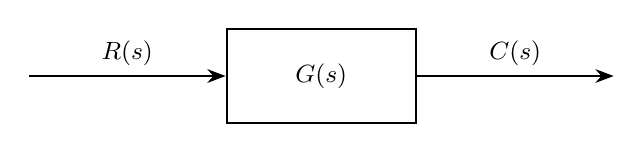
\begin{tikzpicture}[blockdiagram, node distance=1.2cm and 2.5cm]
    \node[input]                        (in)     {};
    \node[block, right=of in]          (ctrl)   {$G(s)$};
    \node[output, right=of ctrl]         (out)    {};
  
    \draw[->] (in) -- node[above] {$R(s)$} (ctrl);
    \draw[->] (ctrl) -- node[above] {$C(s)$} (out);
\end{tikzpicture}
\end{center}
which is equivalent to 
\[C(s) = G(s) \cdot R(s)\]

This could also look like a  \emph{cascade}:
\begin{center}
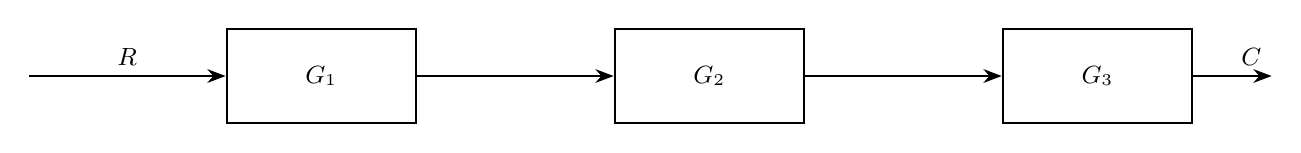
\begin{tikzpicture}[blockdiagram, node distance=0.5cm and 2.5cm]
    \node[input]                        (in)     {};
    \node[block, right=of in]          (ctrl)   {$G_1$};
    \node[block, right=of ctrl]         (act)    {$G_2$};
    \node[block, right=of act]          (plant)  {$G_3$};
    \node[output, right=1cm of plant]   (out)    {};

    \draw[->] (in) -- node[above] {$R$} (ctrl) ;
    \draw[->] (ctrl) -- (act);
    \draw[->] (act) --  (plant);
    \draw[->] (plant) -- (out) node[above left] {$C$};

  
\end{tikzpicture}
\end{center}
\[C = G_1 \cdot G_2 \cdot G_3 \cdot R\]

\tbf{Parallel block diagrams} appear in two forms:
\begin{center}
    \begin{multicols}{2}
        Multi-input:

        \begin{tikzpicture}[blockdiagram]
            \node[sum]                  (sum) {$\sum$};
            \node[input, left=2cm of sum]   (r1)  {};
            \node[input, above=1.2cm of sum] (r2)  {};
            \node[input, below=1.2cm of sum] (r3)  {};
            \node[output, right=2cm of sum]  (out) {};

            \draw[->] (r1) node[left] {$R_1$} -- node[pos=0.85, above] {$+$} (sum);
            \draw[->] (r2) node[above] {$R_2$} -- node[pos=0.85, right] {$+$} (sum);
            \draw[->] (r3) node[below] {$R_3$} -- node[pos=0.85, right] {$-$} (sum);
            \draw[->] (sum) -- node[above] {$C$} (out);
        \end{tikzpicture}
        \[C = R_1 + R_2 - R_3\]

        Multi-path:

        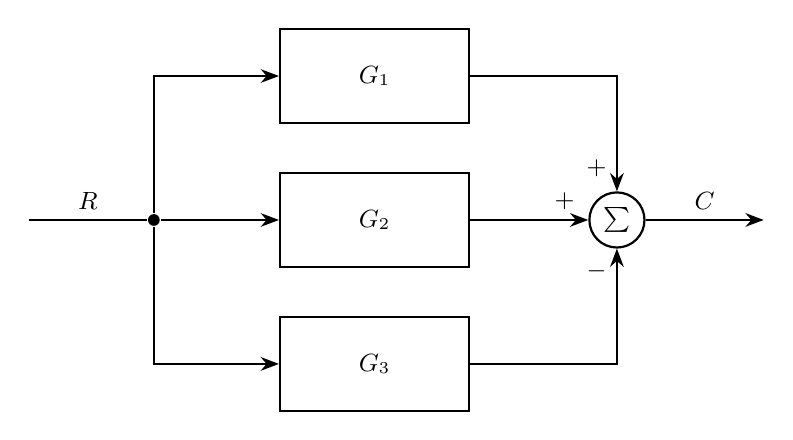
\begin{tikzpicture}[blockdiagram]
            \node[input]                     (in)    {};
            \node[branch, right=1.5cm of in] (split) {};
            \node[block, right=of split]     (g2)    {$G_2$};
            \node[block, above=0.6cm of g2]  (g1)    {$G_1$};
            \node[block, below=0.6cm of g2]  (g3)    {$G_3$};
            \node[sum, right=of g2]          (sum)   {$\sum$};
            \node[output, right=of sum]      (out)   {};

            \draw (in) -- node[above] {$R$} (split);
            \draw[->] (split) |- (g1);
            \draw[->] (split) -- (g2);
            \draw[->] (split) |- (g3);

            \draw[->] (g1) -| node[pos=0.9, left] {$+$} (sum);
            \draw[->] (g2) -- node[pos=0.8, above] {$+$} (sum);
            \draw[->] (g3) -| node[pos=0.9, left] {$-$} (sum);
            \draw[->] (sum) -- node[above] {$C$} (out);
        \end{tikzpicture}
        \[C = (G_1 + G_2 - G_3)R\]
    \end{multicols}
\end{center}

\tbf{Feedback block diagrams} are used to represent systems with feedback loops.

\begin{center}
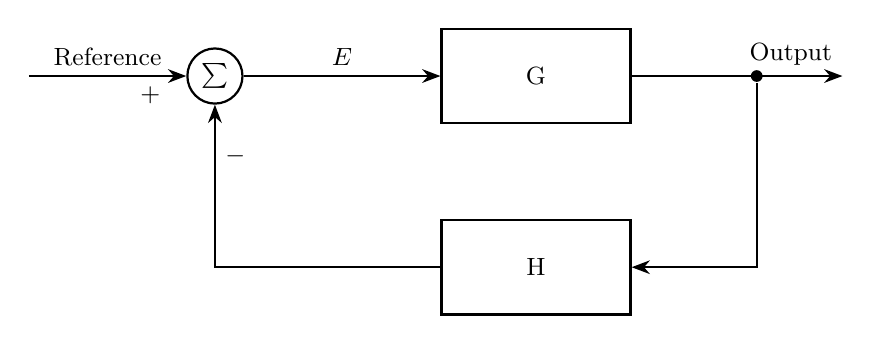
\begin{tikzpicture}[blockdiagram, node distance=1.2cm and 2.5cm]
    \node[input]                        (in)     {};
    \node[sum, right=2cm of in]         (sum)    {$\sum$};
    \node[block, right=of sum]          (ctrl)   {G};
    \node[branch, right=1.5cm of ctrl] (split)  {};
    \node[output, right=1cm of split]   (out)    {};
    \node[block, below=of ctrl]          (sensor) {H};

    \draw[->] (in) -- node[above] {Reference} node[plus] {$+$} (sum);
    \draw[->] (sum) -- node[above] {$E$} (ctrl);
    \draw[->] (ctrl) -- (out) node[above left] {Output};

    \draw[->] (split) |- (sensor);
    \draw[->] (sensor) -| node[minus] {$-$} (sum);
\end{tikzpicture}
\end{center}

What is the transfer function of this system?
\[\begin{cases}
    E = R - CH\\
    C = GE
\end{cases} \implies C = G(R - CH) \implies C = \frac{GR}{1 + GH} \implies \frac{C}{R} = \frac{G}{1 + GH}\]

\section{Sept 24}

\tbf{Recall:} For a block diagram

\begin{center}
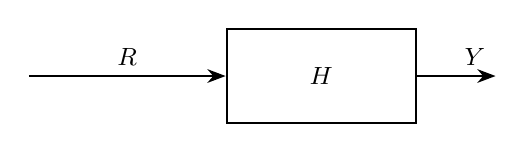
\begin{tikzpicture}[blockdiagram, node distance=1.2cm and 2.5cm]
    \node[input]                        (in)     {};
    \node[block, right=of in]          (ctrl)   {$H$};
    \node[output, right=1cm of ctrl]   (out)    {};

    \draw[->] (in) -- node[above] {$R$} (ctrl);
    \draw[->] (ctrl) -- (out) node[above left] {$Y$};
\end{tikzpicture}
\end{center}

the transfer function is 
\[H(s) = \frac{Y(s)}{R(s)}\]

and the transfer function can be of any order:
\[H(s) = \frac{a_0 s^n + a_1 s^{n-1} + \dots + a_{n-1} s + a_n}{b_0 s^m + b_1 s^{m-1} + \dots + b_{m-1} s + b_m}\]

If $m > n$, we can use partial fractions to decompose the transfer function into a sum of first (a system with real poles) and second order systems (those with complex poles).

If $m = n$, the transfer function will be of the form $H(s) = 1 + \dots$. 

In general, a first order system will nicely converge to a steady state value, while a second order system will oscillate around the steady state value.

\begin{center}
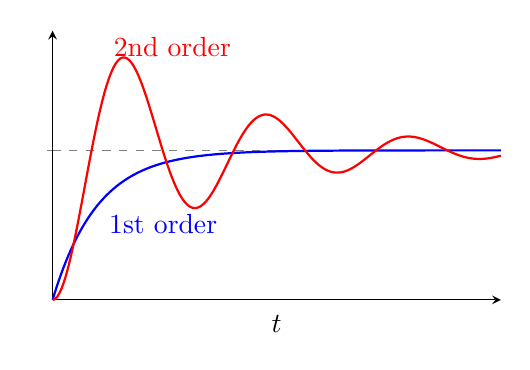
\begin{tikzpicture}
\begin{axis}[
    width=0.6\textwidth, height=5cm,
    axis lines=left,
    no markers,
    xtick=\empty,
    ytick={1},
    yticklabels={},
    xlabel={$t$},
    ylabel={},
    domain=0:10, samples=200,
    xmin=0, xmax=10,
    ymin=0, ymax=1.8,
    clip=false,
]
    \addplot[dashed, gray, domain=0:10, samples=2] {1};
    \addplot[thick, blue] {1 - exp(-x)} node[pos=0.12, below right] {1st order};
    \addplot[thick, red] {1 - exp(-0.3*x)*(cos(deg(1.98*x)) + 0.152*sin(deg(1.98*x)))}
        node[pos=0.16, above right, yshift=2.5ex] {2nd order};
\end{axis}
\end{tikzpicture}
\end{center}

We can always represent the poles of a second order system in the form $s^2 + 2\zeta \omega_n s + \omega_n^2$ for $0 \leq \zeta \leq 1$. (If $\zeta = 1$, the system will have two real poles). 

\begin{exercise}
    \textbf{Exercise:} What is the transfer function of the following system?

    \begin{center}
    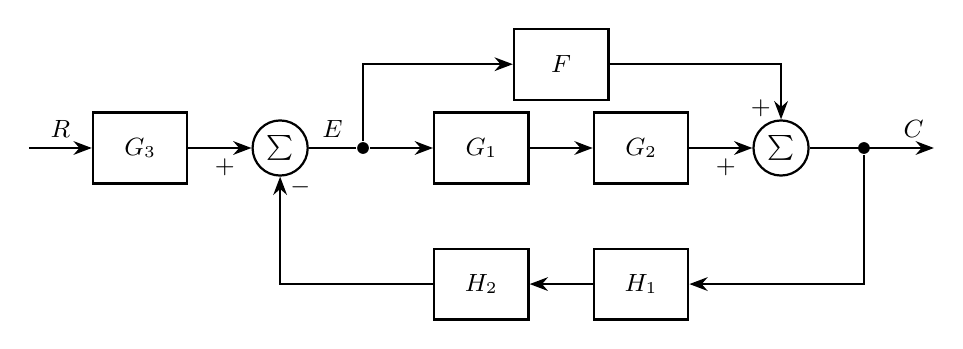
\begin{tikzpicture}[blockdiagram, block/.append style={minimum width=1.2cm, minimum height=0.9cm}, node distance=0.8cm and 0.8cm]
        \node[input]                       (in)     {};
        \node[block, right=of in]          (g3)     {$G_3$};
        \node[sum, right=of g3]            (sum1)   {$\sum$};
        \node[branch, right=0.6cm of sum1] (split1) {};
        \node[block, right=of split1]      (g1)     {$G_1$};
        \node[block, right=of g1]          (g2)     {$G_2$};
        \node[block, above=0.6cm of $(g1)!0.5!(g2)$] (f) {$F$};
        \node[sum, right=of g2]            (sum2)   {$\sum$};
        \node[branch, right=0.6cm of sum2] (split2) {};
        \node[output, right=0.8cm of split2] (out)  {};
        \node[block, below=of g2]          (h1)     {$H_1$};
        \node[block, below=of g1]          (h2)     {$H_2$};

        \draw[->] (in) -- node[above] {$R$} (g3);
        \draw[->] (g3) -- node[plus] {$+$} (sum1);
        \draw (sum1) -- node[above] {$E$} (split1);
        \draw[->] (split1) -- (g1);
        \draw[->] (g1) -- (g2);
        \draw[->] (split1) |- (f);
        \draw[->] (g2) -- node[plus] {$+$} (sum2);
        \draw[->] (f) -| node[pos=0.9, left] {$+$} (sum2);
        \draw[->] (sum2) -- (out) node[above left] {$C$};

        \draw[->] (split2) |- (h1);
        \draw[->] (h1) -- (h2);
        \draw[->] (h2) -| node[pos=0.95, right] {$-$} (sum1);
    \end{tikzpicture}
    \end{center}

       \[\begin{cases}
        E = RG_3 - H_2 H_1 C\\ 
        \begin{aligned}
            C &= EF + EG_1 G_2\\ 
            & = E(F + G_1 G_2)
        \end{aligned} 
    \end{cases}\]

    \begin{align*}
        C &= (RG_3 - H_2 H_1 C)(F + G_1 G_2)\\
        &= RG_3(F + G_1 G_2) - H_2 H_1 C (F + G_1 G_2)\\
        C\left[1 + H_2 H_1 (F + G_1 G_2)\right] &= RG_3(F + G_1 G_2)\\
        \frac{C}{R} &= \frac{G_3(F + G_1 G_2)}{1 + H_2 H_1(F + G_1 G_2)}
    \end{align*}

    We can also use block diagram reduction to simplify the system. First, we can combine $G_1$ and $G_2$ in series, then combine $H_1$ and $H_2$ in series, then combine the two feedback loops into one, and finally combine $G_3$ with the rest of the system in series.

    \begin{center}
    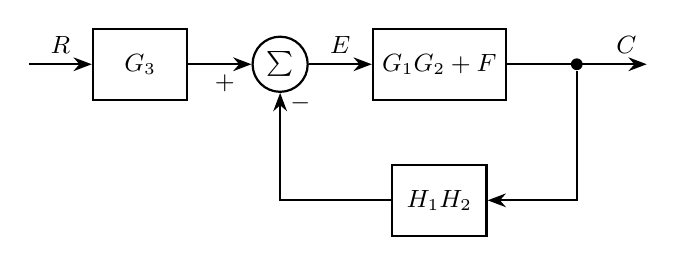
\begin{tikzpicture}[blockdiagram, block/.append style={minimum width=1.2cm, minimum height=0.9cm}, node distance=0.8cm and 0.8cm]
        \node[input]                       (in)    {};
        \node[block, right=of in]          (g3)    {$G_3$};
        \node[sum, right=of g3]            (sum)   {$\sum$};
        \node[block, right=of sum]         (fwd)   {$G_1G_2 + F$};
        \node[branch, right=0.8cm of fwd]  (split) {};
        \node[output, right=0.8cm of split] (out)  {};
        \node[block, below=of fwd]         (fb)    {$H_1H_2$};

        \draw[->] (in) -- node[above] {$R$} (g3);
        \draw[->] (g3) -- node[plus] {$+$} (sum);
        \draw[->] (sum) -- node[above] {$E$} (fwd);
        \draw[->] (fwd) -- (out) node[above left] {$C$};

        \draw[->] (split) |- (fb);
        \draw[->] (fb) -| node[pos=0.95, right] {$-$} (sum);
    \end{tikzpicture}
    \end{center}

    Which, using the general formula, gives 
    \[\frac{C}{G_3R} = \frac{F + G_1G_2}{1 + (H_1H_2)(F + G_1G_2)} \implies \frac{C}{R} = \frac{G_3(F + G_1G_2)}{1 + (H_1H_2)(F + G_1G_2)}\]
\end{exercise}

In the example above, we call the $F$ branch a \emph{feedforward} branch, while the $H_1H_2$ branch is a \emph{feedback} branch. $G_1G_2$ is assumed to be the \emph{plant control}.

\begin{exercise}
    \textbf{Exercise:} Find the transfer function of the system 
       \begin{center}
    \begin{tikzpicture}[blockdiagram, block/.append style={minimum width=1.2cm, minimum height=0.9cm}, node distance=0.8cm and 0.8cm]
        \node[input]                       (in)    {};
        \node[sum, right=of g3]            (sum)   {$\sum$};
        \node[block, right=of sum]         (fwd)   {$G_1 + F$};
        \node[branch, right=0.8cm of fwd]  (split) {};
        \node[output, right=0.8cm of split] (out)  {};
        \node[block, below=of fwd]         (fb)    {$H_2$};

        \draw[->] (in) -- node[above] {$R$} (g3);
        \draw[->] (g3) -- node[plus] {$+$} (sum);
        \draw[->] (sum) -- node[above] {$E$} (fwd);
        \draw[->] (fwd) -- (out) node[above left] {$C$};

        \draw[->] (split) |- (fb);
        \draw[->] (fb) -| node[pos=0.95, right] {$-$} (sum);
    \end{tikzpicture}
    \end{center}
    where $F = 1$, $G_1 = \frac{5}{s + 5}$, $H_2 = \frac{7}{s + 7}$,

    \begin{align*}
        \frac{C}{R} &= \frac{G_1 + F}{1 + H_2(G_1 + F)}\\
        &= \frac{\frac{5}{s + 5} + 1}{1 + \frac{7}{s + 7}\left(\frac{5}{s + 5} + 1\right)}\\
        &= \frac{\frac{5 + s + 5}{s + 5}}{\frac{(s + 7)(s + 5) + 7(5 + s + 5)}{(s + 7)(s + 5)}}\\
        &= \frac{(s + 7)(s + 10)}{(s + 7)(s + 5) + 7(s + 10)}\\
        &= \frac{(s+7)(s+10)}{s^2 + 19s + 105}
    \end{align*}
\end{exercise}

\begin{exercise}
    \textbf{Exercise:} Find the transfer function of the system

    \begin{center}
    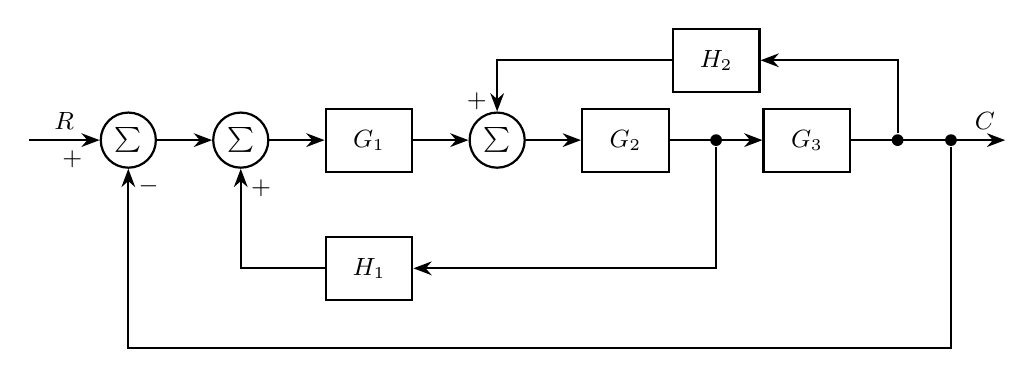
\begin{tikzpicture}[blockdiagram, block/.append style={minimum width=1.1cm, minimum height=0.8cm}, node distance=0.8cm and 0.7cm]
        \node[input]                         (in)    {};
        \node[sum, right=0.9cm of in]        (sum1)  {$\sum$};
        \node[sum, right=of sum1]            (sum2)  {$\sum$};
        \node[block, right=of sum2]          (g1)    {$G_1$};
        \node[sum, right=of g1]              (sum3)  {$\sum$};
        \node[block, right=of sum3]          (g2)    {$G_2$};
        \node[branch, right=0.5cm of g2]     (pm)    {};
        \node[block, right=0.5cm of pm]      (g3)    {$G_3$};
        \node[branch, right=0.5cm of g3]     (p1)    {};
        \node[branch, right=0.5cm of p1]     (p3)    {};
        \node[output, right=0.6cm of p3]     (out)   {};
        \node[block, above=0.6cm of $(g2)!0.5!(g3)$] (h2) {$H_2$};
        \node[block, below=of g1]            (h1)    {$H_1$};

        \draw[->] (in) -- node[above] {$R$} node[plus] {$+$} (sum1);
        \draw[->] (sum1) -- (sum2);
        \draw[->] (sum2) -- (g1);
        \draw[->] (g1) -- (sum3);
        \draw[->] (sum3) -- (g2);
        \draw[->] (g2) -- (g3);
        \draw[->] (g3) -- (out) node[above left] {$C$};

        % inner loop
        \draw[->] (p1) |- (h2);
        \draw[->] (h2) -| node[pos=0.9, left] {$+$} (sum3);

        % middle loop (picked off between G_2 and G_3)
        \draw[->] (pm) |- (h1);
        \draw[->] (h1) -| node[pos=0.9, right] {$+$} (sum2);

        % outer loop
        \draw[->] (p3) |- ($(h1.south)+(0,-0.6)$) -| node[pos=0.95, right] {$-$} (sum1);
    \end{tikzpicture}
    \end{center}

    The trick is to simplify: 

    \begin{center}
    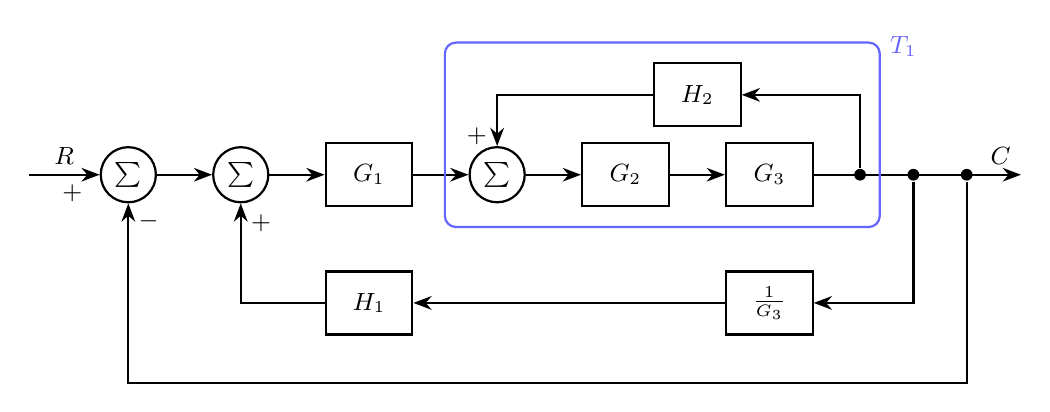
\begin{tikzpicture}[blockdiagram, block/.append style={minimum width=1.1cm, minimum height=0.8cm}, node distance=0.8cm and 0.7cm]
        \node[input]                         (in)    {};
        \node[sum, right=0.9cm of in]        (sum1)  {$\sum$};
        \node[sum, right=of sum1]            (sum2)  {$\sum$};
        \node[block, right=of sum2]          (g1)    {$G_1$};
        \node[sum, right=of g1]              (sum3)  {$\sum$};
        \node[block, right=of sum3]          (g2)    {$G_2$};
        \node[block, right=of g2]            (g3)    {$G_3$};
        \node[branch, right=0.5cm of g3]     (p1)    {};
        \node[branch, right=0.5cm of p1]     (p2)    {};
        \node[branch, right=0.5cm of p2]     (p3)    {};
        \node[output, right=0.6cm of p3]     (out)   {};
        \node[block, above=0.6cm of $(g2)!0.5!(g3)$] (h2) {$H_2$};
        \node[block, below=of g3]            (ig3)   {$\frac{1}{G_3}$};
        \node[block, below=of g1]            (h1)    {$H_1$};

        \draw[->] (in) -- node[above] {$R$} node[plus] {$+$} (sum1);
        \draw[->] (sum1) -- (sum2);
        \draw[->] (sum2) -- (g1);
        \draw[->] (g1) -- (sum3);
        \draw[->] (sum3) -- (g2);
        \draw[->] (g2) -- (g3);
        \draw[->] (g3) -- (out) node[above left] {$C$};

        % inner loop
        \draw[->] (p1) |- (h2);
        \draw[->] (h2) -| node[pos=0.9, left] {$+$} (sum3);

        % middle loop
        \draw[->] (p2) |- (ig3);
        \draw[->] (ig3) -- (h1);
        \draw[->] (h1) -| node[pos=0.9, right] {$+$} (sum2);

        % outer loop
        \draw[->] (p3) |- ($(h1.south)+(0,-0.6)$) -| node[pos=0.95, right] {$-$} (sum1);

        % inner loop outline
        \draw[blue!60, rounded corners] ($(sum3.west |- h2.north)+(-0.3,0.25)$) rectangle ($(p1 |- g3.south)+(0.25,-0.25)$) node[above right, yshift=0.8in] {$T_1$};
    \end{tikzpicture}
    \end{center}

    Inner block:
    \[T_1  = \frac{G_2 G_3}{1 - G_2 G_3 H_2}\]
    (notice the flipped sign in the denominator because the feedback is positive).

    \begin{center}
    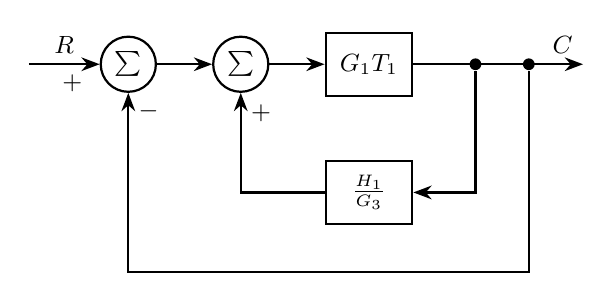
\begin{tikzpicture}[blockdiagram, block/.append style={minimum width=1.1cm, minimum height=0.8cm}, node distance=0.8cm and 0.7cm]
        \node[input]                         (in)    {};
        \node[sum, right=0.9cm of in]        (sum1)  {$\sum$};
        \node[sum, right=of sum1]            (sum2)  {$\sum$};
        \node[block, right=of sum2]          (t1)    {$G_1T_1$};
        \node[branch, right=0.7cm of t1]     (p2)    {};
        \node[branch, right=0.5cm of p2]     (p3)    {};
        \node[output, right=0.6cm of p3]     (out)   {};
        \node[block, below=of t1]            (h1)    {$\frac{H_1}{G_3}$};

        \draw[->] (in) -- node[above] {$R$} node[plus] {$+$} (sum1);
        \draw[->] (sum1) -- (sum2);
        \draw[->] (sum2) -- (t1);
        \draw[->] (t1) -- (out) node[above left] {$C$};

        % middle loop
        \draw[->] (p2) |- (h1);
        \draw[->] (h1) -| node[pos=0.9, right] {$+$} (sum2);

        % outer loop
        \draw[->] (p3) |- ($(h1.south)+(0,-0.6)$) -| node[pos=0.95, right] {$-$} (sum1);
    \end{tikzpicture}
    \end{center}

    Then letting,
    \[T_2 = \frac{H_1}{G_3}\]
    we have 
    \[T_3 = \frac{G_1 T_1}{1 - G_1 T_1 T_2}\]

    \begin{center}
    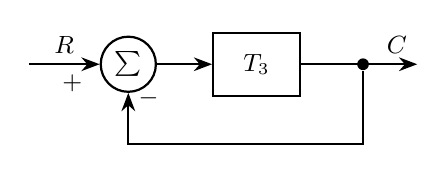
\begin{tikzpicture}[blockdiagram, block/.append style={minimum width=1.1cm, minimum height=0.8cm}, node distance=0.8cm and 0.7cm]
        \node[input]                         (in)    {};
        \node[sum, right=0.9cm of in]        (sum1)  {$\sum$};
        \node[block, right=of sum1]          (t3)    {$T_3$};
        \node[branch, right=0.7cm of t3]     (p3)    {};
        \node[output, right=0.6cm of p3]     (out)   {};

        \draw[->] (in) -- node[above] {$R$} node[plus] {$+$} (sum1);
        \draw[->] (sum1) -- (t3);
        \draw[->] (t3) -- (out) node[above left] {$C$};

        % outer loop
        \draw[->] (p3) |- ($(t3.south)+(0,-0.6)$) -| node[pos=0.95, right] {$-$} (sum1);
    \end{tikzpicture}
    \end{center}

    And finally, 
    \[\frac{C}{R} = \frac{T_3}{1 + T_3}\]

\end{exercise}

As you can see, block diagram reduction is a very useful tool for simplifying complex systems. It allows us to break down the system into smaller, more manageable parts, and then combine them to find the overall transfer function. However, this is still a very tedious process, and it is easy to make mistakes.

Let's use Matlab instead. 

\tbf{Example:}
\begin{center}
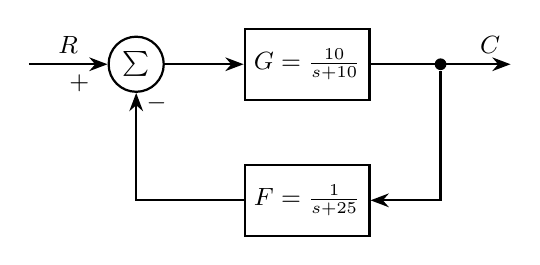
\begin{tikzpicture}[blockdiagram, block/.append style={minimum width=1.4cm, minimum height=0.9cm}, node distance=0.8cm and 1cm]
    \node[input]                         (in)    {};
    \node[sum, right=of in]              (sum)   {$\sum$};
    \node[block, right=of sum]           (g)     {$G = \frac{10}{s + 10}$};
    \node[branch, right=0.8cm of g]      (split) {};
    \node[output, right=0.8cm of split]  (out)   {};
    \node[block, below=of g]             (f)     {$F = \frac{1}{s + 25}$};

    \draw[->] (in) -- node[above] {$R$} node[plus] {$+$} (sum);
    \draw[->] (sum) -- (g);
    \draw[->] (g) -- (out) node[above left] {$C$};

    \draw[->] (split) |- (f);
    \draw[->] (f) -| node[pos=0.95, right] {$-$} (sum);
\end{tikzpicture}
\end{center}

\begin{lstlisting}
    s = tf('s');
    G = 10/(s + 10); 

    step(G) % gets the step response of the system
    impulse(G) % gets the impulse response of the system

    F = 1/(s + 25); 
    CLTF = feedback(G, F) % gets the closed loop transfer function of the system
\end{lstlisting}

This will output 
\[\tt{CLTF} = \frac{10s + 250}{s^2 + 35s + 250}\]

\tbf{Example:} 

    \begin{center}
    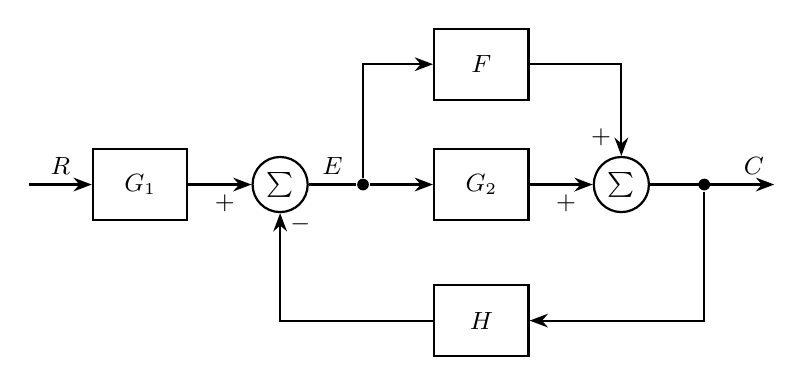
\begin{tikzpicture}[blockdiagram, block/.append style={minimum width=1.2cm, minimum height=0.9cm}, node distance=0.8cm and 0.8cm]
        \node[input]                       (in)     {};
        \node[block, right=of in]          (g3)     {$G_1$};
        \node[sum, right=of g3]            (sum1)   {$\sum$};
        \node[branch, right=0.6cm of sum1] (split1) {};
        \node[block, right=of split1]      (g12)    {$G_2$};
        \node[block, above=0.6cm of g12]   (f)      {$F$};
        \node[sum, right=of g12]           (sum2)   {$\sum$};
        \node[branch, right=0.6cm of sum2] (split2) {};
        \node[output, right=0.8cm of split2] (out)  {};
        \node[block, below=of g12]         (h12)    {$H$};

        \draw[->] (in) -- node[above] {$R$} (g3);
        \draw[->] (g3) -- node[plus] {$+$} (sum1);
        \draw (sum1) -- node[above] {$E$} (split1);
        \draw[->] (split1) -- (g12);
        \draw[->] (split1) |- (f);
        \draw[->] (g12) -- node[plus] {$+$} (sum2);
        \draw[->] (f) -| node[pos=0.9, left] {$+$} (sum2);
        \draw[->] (sum2) -- (out) node[above left] {$C$};

        \draw[->] (split2) |- (h12);
        \draw[->] (h12) -| node[pos=0.95, right] {$-$} (sum1);
    \end{tikzpicture}
    \end{center}

    We can define $Q_1 = F + G_2$ so the system can be solved with 
    \begin{lstlisting}
        s = tf('s');
        syms F G1 G2 H; 
        Q = G + G2; 

        M = feedback(Q, H); 
        CLTF = Series(M, G1)       

        ltview(CLTF) %  opens the linear system analyzer
\end{lstlisting}

\begin{exercise}
    \textbf{Exercise:}  Find $\frac{C}{R}$ for the system

\begin{center}
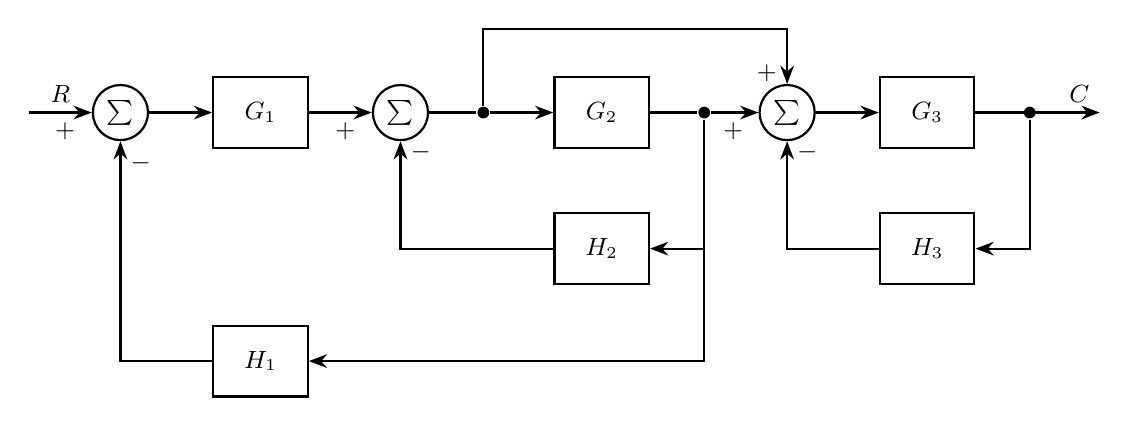
\begin{tikzpicture}[blockdiagram, block/.append style={minimum width=1.2cm, minimum height=0.9cm}, node distance=0.8cm and 0.8cm]
    \node[input]                          (in)    {};
    \node[sum, right=of in]               (sum1)  {$\sum$};
    \node[block, right=of sum1]           (g1)    {$G_1$};
    \node[sum, right=of g1]               (sum2)  {$\sum$};
    \node[branch, right=0.6cm of sum2]    (pa)    {};
    \node[block, right=of pa]             (g2)    {$G_2$};
    \node[branch, right=0.6cm of g2]      (pb)    {};
    \node[sum, right=0.6cm of pb]         (sum3)  {$\sum$};
    \node[block, right=of sum3]           (g3)    {$G_3$};
    \node[branch, right=0.6cm of g3]      (pc)    {};
    \node[output, right=0.8cm of pc]      (out)   {};
    \node[block, below=of g2]             (h2)    {$H_2$};
    \node[block, below=0.5cm of h2.south -| g1] (h1) {$H_1$};
    \node[block, below=of g3]             (h3)    {$H_3$};

    \draw[->] (in) -- node[above] {$R$} node[plus] {$+$} (sum1);
    \draw[->] (sum1) -- (g1);
    \draw[->] (g1) -- node[plus] {$+$} (sum2);
    \draw (sum2) -- (pa);
    \draw[->] (pa) -- (g2);
    \draw (g2) -- (pb);
    \draw[->] (pb) -- node[plus] {$+$} (sum3);
    \draw[->] (sum3) -- (g3);
    \draw[->] (g3) -- (out) node[above left] {$C$};

    % feedforward around G_2
    \draw[->] (pa) |- ($(g2.north)+(0,0.6)$) -| node[pos=0.9, left] {$+$} (sum3);

    % H_2 and H_1 picked off after G_2
    \draw[->] (pb) |- (h2);
    \draw[->] (h2) -| node[pos=0.95, right] {$-$} (sum2);
    \draw[->] (pb) |- (h1);
    \draw[->] (h1) -| node[pos=0.95, right] {$-$} (sum1);

    % H_3 around G_3
    \draw[->] (pc) |- (h3);
    \draw[->] (h3) -| node[pos=0.95, right] {$-$} (sum3);
\end{tikzpicture}
\end{center}

Letting
\[T_1 = \frac{G_2}{1 + G_2H_2}\]
and moving the feedforward branch to after $T_1$, we have

\begin{center}
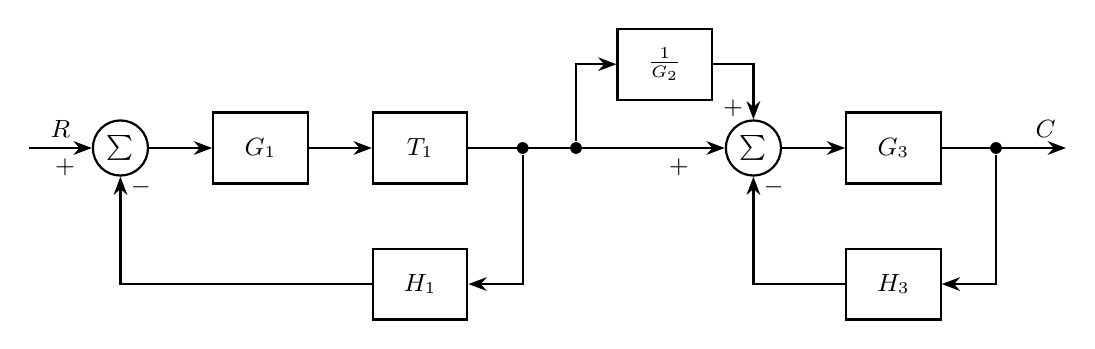
\begin{tikzpicture}[blockdiagram, block/.append style={minimum width=1.2cm, minimum height=0.9cm}, node distance=0.8cm and 0.8cm]
    \node[input]                          (in)    {};
    \node[sum, right=of in]               (sum1)  {$\sum$};
    \node[block, right=of sum1]           (g1)    {$G_1$};
    \node[block, right=of g1]             (t1)    {$T_1$};
    \node[branch, right=0.6cm of t1]      (pb)    {};
    \node[branch, right=0.5cm of pb]      (pf)    {};
    \node[sum, right=1.8cm of pf]         (sum3)  {$\sum$};
    \node[block, above=0.6cm of $(pf)!0.5!(sum3)$] (ig2) {$\frac{1}{G_2}$};
    \node[block, right=of sum3]           (g3)    {$G_3$};
    \node[branch, right=0.6cm of g3]      (pc)    {};
    \node[output, right=0.8cm of pc]      (out)   {};
    \node[block, below=of t1]             (h1)    {$H_1$};
    \node[block, below=of g3]             (h3)    {$H_3$};

    \draw[->] (in) -- node[above] {$R$} node[plus] {$+$} (sum1);
    \draw[->] (sum1) -- (g1);
    \draw[->] (g1) -- (t1);
    \draw[->] (t1) -- node[plus] {$+$} (sum3);
    \draw[->] (sum3) -- (g3);
    \draw[->] (g3) -- (out) node[above left] {$C$};

    % feedforward, pickoff moved past G_2
    \draw[->] (pf) |- (ig2);
    \draw[->] (ig2) -| node[pos=0.9, left] {$+$} (sum3);

    % H_1 picked off after T_1
    \draw[->] (pb) |- (h1);
    \draw[->] (h1) -| node[pos=0.95, right] {$-$} (sum1);

    % H_3 around G_3
    \draw[->] (pc) |- (h3);
    \draw[->] (h3) -| node[pos=0.95, right] {$-$} (sum3);
\end{tikzpicture}
\end{center}

With 
\[T_2 = \frac{T_1 G_1}{1 + T_1 G_1 H_1}\]
the first section simplifies into a single block:


\begin{center}
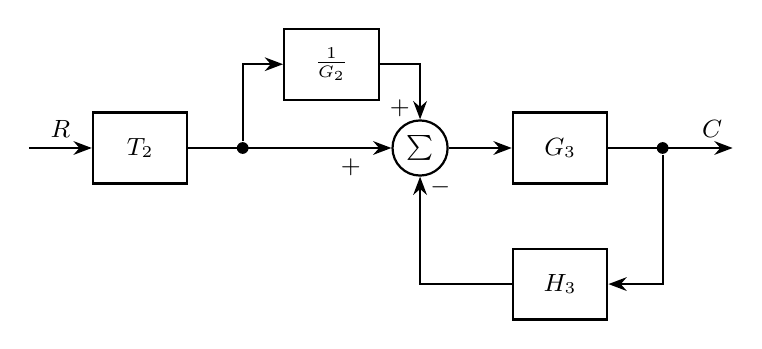
\begin{tikzpicture}[blockdiagram, block/.append style={minimum width=1.2cm, minimum height=0.9cm}, node distance=0.8cm and 0.8cm]
    \node[input]                          (in)    {};
    \node[block, right=of in]             (t2)    {$T_2$};
    \node[branch, right=0.6cm of t2]      (pf)    {};
    \node[sum, right=1.8cm of pf]         (sum3)  {$\sum$};
    \node[block, above=0.6cm of $(pf)!0.5!(sum3)$] (ig2) {$\frac{1}{G_2}$};
    \node[block, right=of sum3]           (g3)    {$G_3$};
    \node[branch, right=0.6cm of g3]      (pc)    {};
    \node[output, right=0.8cm of pc]      (out)   {};
    \node[block, below=of g3]             (h3)    {$H_3$};

    \draw[->] (in) -- node[above] {$R$} (t2);
    \draw[->] (t2) -- node[plus] {$+$} (sum3);
    \draw[->] (sum3) -- (g3);
    \draw[->] (g3) -- (out) node[above left] {$C$};

    % feedforward
    \draw[->] (pf) |- (ig2);
    \draw[->] (ig2) -| node[pos=0.9, left] {$+$} (sum3);

    % H_3 around G_3
    \draw[->] (pc) |- (h3);
    \draw[->] (h3) -| node[pos=0.95, right] {$-$} (sum3);
\end{tikzpicture}
\end{center}

And finally, 
\[T_3 = \frac{G_3}{1 + G_3 H_3}\]
gives a simple parallel-series system to be solved by matlab:

\begin{center}
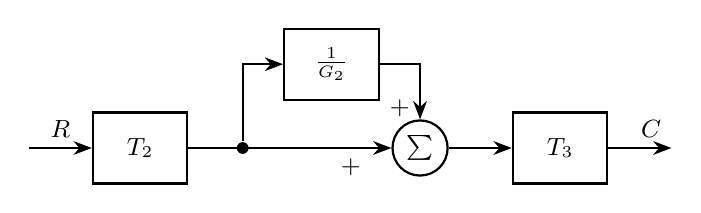
\begin{tikzpicture}[blockdiagram, block/.append style={minimum width=1.2cm, minimum height=0.9cm}, node distance=0.8cm and 0.8cm]
    \node[input]                          (in)    {};
    \node[block, right=of in]             (t2)    {$T_2$};
    \node[branch, right=0.6cm of t2]      (pf)    {};
    \node[sum, right=1.8cm of pf]         (sum3)  {$\sum$};
    \node[block, above=0.6cm of $(pf)!0.5!(sum3)$] (ig2) {$\frac{1}{G_2}$};
    \node[block, right=of sum3]           (t3)    {$T_3$};
    \node[output, right=of t3]            (out)   {};

    \draw[->] (in) -- node[above] {$R$} (t2);
    \draw[->] (t2) -- node[plus] {$+$} (sum3);
    \draw[->] (sum3) -- (t3);
    \draw[->] (t3) -- (out) node[above left] {$C$};

    % feedforward
    \draw[->] (pf) |- (ig2);
    \draw[->] (ig2) -| node[pos=0.9, left] {$+$} (sum3);
\end{tikzpicture}
\end{center}

\end{exercise}


\section{Sept 29}

We can view a system

\begin{center}
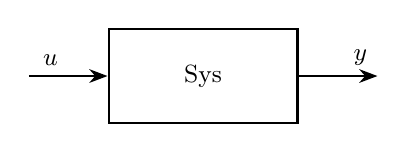
\begin{tikzpicture}[blockdiagram, node distance=1.2cm and 2.5cm]
    \node[input]                        (in)     {};
    \node[block, right=1cm of in]          (ctrl)   {Sys};
    \node[output, right=1cm of ctrl]   (out)    {};

    \draw[->] (in) -- node[above left] {$u$} (ctrl);
    \draw[->] (ctrl) -- (out) node[above left] {$y$};
\end{tikzpicture}
\end{center}

in three ways:
\begin{enumerate}
    \item Differential Equations (e.g. $\ddot y + 2t\dot y + y = u$ which cannot be solved via Laplace because it is not LTI)
    \item Transfer function (e.g. $\frac{Y}{U} = \frac{s+1}{s^2 + 4s + 11}$)
    \item State space (e.g. $\dot X = Ax + bu,\; Y = cx + du$) 
\end{enumerate}

As it happens, during the Space Race, the Americans were using transfer functions which excelled at single-input, single-output systems. For Sputnik, Lyapunov developed the state-space formulation which can handle \emph{multi-input, multi-output systems.}

\tbf{Example (converting to state space):} Recall the spring-mass-damper system. 

\begin{center}
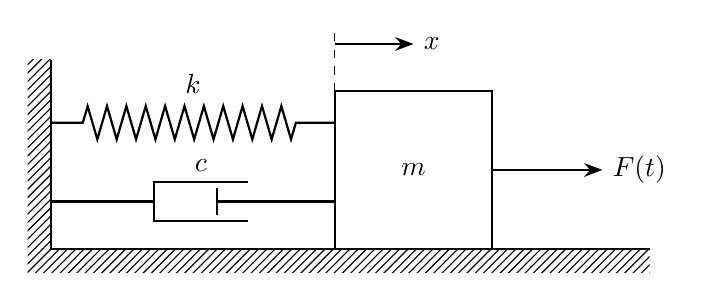
\begin{tikzpicture}[>=Stealth, thick]
    % wall and ground
    \fill[pattern=north east lines] (-0.3,0) rectangle (0,2.4);
    \fill[pattern=north east lines] (-0.3,-0.3) rectangle (7.6,0);
    \draw (0,2.4) -- (0,0) -- (7.6,0);

    % mass
    \draw (3.6,0) rectangle ++(2,2) node[midway] {$m$};

    % spring
    \draw[decoration={zigzag, segment length=7pt, amplitude=6pt, pre length=0.4cm, post length=0.4cm}, decorate]
        (0,1.6) -- (3.6,1.6) node[midway, above=7pt] {$k$};

    % damper
    \draw (0,0.6) -- (1.3,0.6);
    \draw (2.5,0.35) -- (1.3,0.35) -- (1.3,0.85) -- (2.5,0.85);
    \draw (2.1,0.43) -- (2.1,0.77);
    \draw (2.1,0.6) -- (3.6,0.6);
    \node[above] at (1.9,0.85) {$c$};

    % force
    \draw[->] (5.6,1) -- ++(1.4,0) node[right] {$F(t)$};

    % displacement
    \draw[dashed, thin] (3.6,2) -- (3.6,2.8);
    \draw[->] (3.6,2.6) -- ++(1,0) node[right] {$x$};
\end{tikzpicture}
\end{center}

\[m\ddot x + c\dot x + kx = f\]

We want to write this system as a state-space system of the form 
\[\begin{cases}
    \dot X = Ax + bu\\ 
    Y = cx + du
\end{cases}\]

In general, the order of the differential equation will dictate the size of the matrix $A$. 

For a second-order ODE, $A \in \R^{2 \times 2}$, $u \in \R^{2\times 1}, c \in \R^{1 \times 2}, d \in \R^{1 \times 1}, x \in \R^{2\times 1}$. 

Define a \tbf{state variable}
\[X = \begin{pmatrix}
    x_1\\x_2
\end{pmatrix}\]
and suppose $x_1 = x$ (the position of the mass) and $x_2 = \dot x$ (the velocity). 

In particular, this means 
\[\dot x_1 = x_2\]
so 
\[\ddot x = \frac{1}{m}(f - c\dot x - kx) \implies \dot x_2 = \frac{1}{m}(f - cx_2 - kx_1)\]
hence 
\begin{align*}
    \begin{bmatrix}
        \dot x_1\\ \dot x_2
    \end{bmatrix} &= \overbrace{\begin{bmatrix}
        0 & 1\\ 
        -\frac{k}{m} & -\frac{c}{m}
    \end{bmatrix}}^A \begin{bmatrix}
        x_1\\ x_2
    \end{bmatrix} + \overbrace{\begin{bmatrix}
        0\\ \frac{1}{m}
    \end{bmatrix}}^B f\\ 
    Y &= \underbrace{\begin{bmatrix}
        1 & 0
    \end{bmatrix}}_C \begin{bmatrix}
        x_1\\ x_2
    \end{bmatrix}
\end{align*}
(making the arbitrary choice that we want the position as our output)

If instead we wanted $[x, \dot x]$ as our output, we could define 
\[Y = \begin{bmatrix}
        1 & 0\\ 
        0 & 1
    \end{bmatrix} \begin{bmatrix}
        x_1\\ x_2
    \end{bmatrix}\]

This method lets us move from DiffEq to state space. How do we move from state space to transfer function or transfer function to state space?

Trivially, to move from transfer function to state space just cross-multiply to recover the ODE and then move the state space. 

The more difficult direction is state space to transfer function. Just take the Laplace and solve for $Y/U$.

First, solving for $X(s)$:
\begin{gather*}
     s X(s) = AX(s) + BU(s)\\ 
    (sI - A)X(s) = BU(s)\\ 
    X(s) = (sI-A)^{-1} BU(s)\\ 
\end{gather*}

Then, substituting, 
\begin{align*}
    Y(s) &= CX(s) + DU(s)\\ 
    &= (C(sI - A)^{-1} B + D)U(s)
\end{align*}
which gives the general form 
\[\boxed{\frac{Y(s)}{U(s)} = C(sI - A)^{-1} B + D}\]

In our example, 
\begin{align*}
    (sI - A) &= \begin{bmatrix}
        s & -1\\ 
        \frac{k}{m} & s + \frac{c}{m}
    \end{bmatrix}\\ 
    (sI- A)^{-1} &= \frac{1}{s(s + \frac{c}{m}) + \frac{k}{m}} \begin{bmatrix}
        s + \frac{c}{m} & 1\\ 
        -\frac{k}{m} & s
    \end{bmatrix}\\ 
    \frac{Y(s)}{U(s)} &=  C(sI - A)^{-1} B + D\\ 
    &=  \frac{1}{s^2 + \frac{cs}{m} + \frac{k}{m}} \begin{bmatrix}
        1 & 0
    \end{bmatrix}\begin{bmatrix}
        s + \frac{c}{m} & 1\\ 
        -\frac{k}{m} & s
    \end{bmatrix} \begin{bmatrix}
        0 \\ \frac{1}{m}
    \end{bmatrix}\\ 
    &=  \frac{1}{s^2 + \frac{cs}{m} + \frac{k}{m}} \begin{bmatrix}
        1 & 0
    \end{bmatrix} \begin{bmatrix}
        \frac{1}{m} \\ \frac{s}{m}
    \end{bmatrix}\\ 
    &=   \frac{1}{ms^2 + cs + k} 
\end{align*}

Which is exactly what we found via Laplace:
\[m\ddot x + c\dot x + kx = f \implies ms^2X(s) + csX(s) + kX(s) = F \implies \frac{X(s)}{F(s)} = \frac{1}{ms^2 + cs + k}\] 

The general \tbf{non-linear state space form} is 
\[\begin{cases}
    \dot x = f(x, u)\\ 
    y = h(x, u)
\end{cases}\]

Nonlinear systems can be controlled either via \tbf{linearization} or \tbf{non-linear control}. Only linearization will be treated in this course. 

Two basic methods: make a linear approximation (e.g. $\sin \theta = \theta$) or linearize around equilibria.

\emph{Example:} Consider a transatlantic flight. Over the length of the flight, fuel usage can lead to a change in mass of almost 40\%. We would like our controller to respond to this change without needing to model the system continuously. 

We can take advantage of times when the plane has constant speed (e.g. no acceleration) to solve for equilibria 
\[\begin{cases}
    \dot x = 0\\ 
    f(x, u) \big\vert_{x_0, u_0} = 0\\ 
    y = h(x_0, y_0)
\end{cases} \implies \begin{matrix}
    A = \frac{\partial f}{\partial x}\big\vert_{u_0, x_0} & 
    C = \frac{\partial h}{\partial x}\big\vert_{u_0, x_0}\\ \\
    B = \frac{\partial f}{\partial u}\big\vert_{u_0, x_0} & 
    D = \frac{\partial h}{\partial u}\big\vert_{u_0, x_0}\\
\end{matrix}\]
in a higher dimensional analogue to  
\[f(x) = f(x_0) + \frac{\partial f}{\partial x}\bigg\vert_{x_0} (x - x_0)\]
\end{document}